
\section{Introduction}

Solar cells is an important renewable energy source. Solar energy has the potential to solve challenges related to renewable energy with regards to climate issues. A prognoses done by Bundesverband Solarwirthschaft for German solar industry, suggest that solar energy will dominate the energy section 100 years from now. To realize this, larger production volumes, and better utilization of the sunlight is needed. Photovoltaic solar cells generating electricity are dominated by multicrystalline silicon fabrication. This gives cost efficient solar cells, but at a low efficiency. The low efficiency makes for a large potential increase. In order to increase efficiency, it is important to understand how a solar cell works, and efficiently be able to characterize solar cell materials.

\begin{figure}[H]
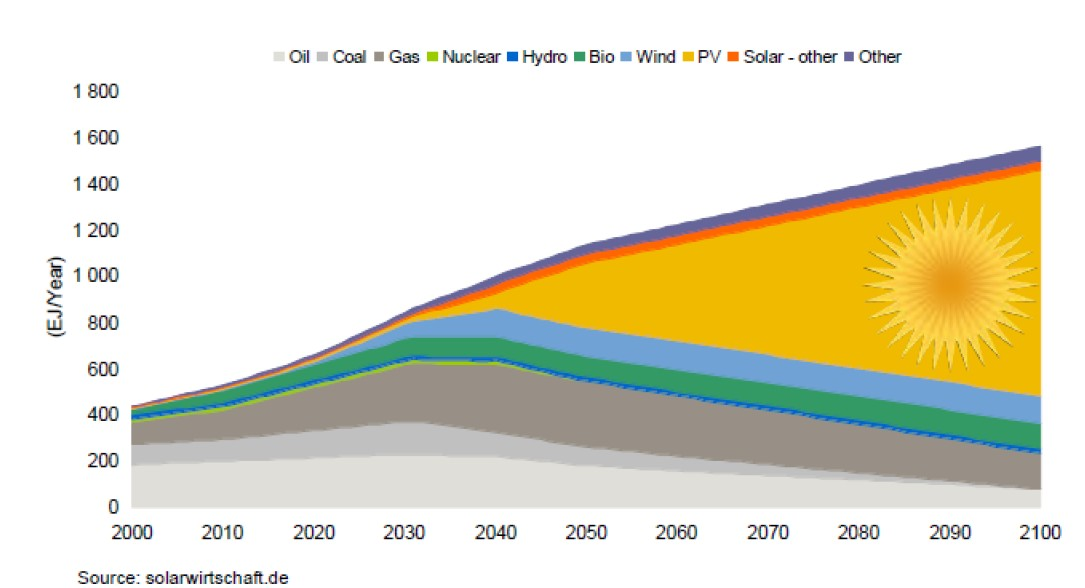
\includegraphics[width=\columnwidth]{enery_mix}%
\caption{Prognose for yearly energy production}%
\label{fig:energimix}%
\end{figure}

This thesis is concentrating about silicon characterization based on photoluminescence at low temperatures. By illuminating a sample of multicrystalline silicon, it is possible to extract information about the sample based on the returning light. Even small concentrations of impurities will influence the properties of silicon material, and hence the solar cell. 

An overview of previous studies characterizing relevant spectra for silicon is needed, as well as an understanding of how photoluminescence can be used to detect and characterize different defects and impurities. 

Three different samples has been chosen. One clean sample with few impurities, and two samples from a compensated feedstock. These samples are from wafers produced by the photovoltaic industry (the compensated feedstock samples are from Elkem), and consist of multicrystalline silicon. The goal is to characterize these three samples by the use of low temperature micro photoluminescence.